\documentclass[31pt]{article}
\setlength{\columnsep}{0.13\columnwidth}
%\setlength{\columnseprule}{0.05\columnwidth}
 
\usepackage{geometry}
\geometry{left=2.3cm, right=2.3cm, top=2.5cm, bottom=2.5cm}

\usepackage{fontspec}
\setmainfont{Times New Roman}

\usepackage{xeCJK}

\usepackage{subfigure}

\usepackage{amssymb}

\usepackage{amsmath}

\usepackage{graphicx}

\usepackage{booktabs}

\usepackage{longtable}

\usepackage{tabularx}

\usepackage{wrapfig}

\usepackage{indentfirst}

\usepackage{bm}								%粗斜体

\usepackage{float}								%超级好用!浮动排版!

\usepackage{flushend,cuted}
 
\usepackage{caption}
\captionsetup{font={scriptsize}}						%改变图名字体大小

\usepackage{subfig}
\captionsetup[subfigure]{labelformat=simple, listofformat=subsimple, farskip = 0pt}

\usepackage{hyperref}							%超链接!

\usepackage{fancyhdr}

\usepackage{stfloats}

\setlength{\parindent}{2em}

\linespread{1.2}

\usepackage{ragged2e}             %两端对齐!

\usepackage{algorithm}

\usepackage{algorithmicx}

\usepackage{algpseudocode}

\renewcommand{\algorithmicrequire}{\textbf{Input:}}  % Use Input in the format of Algorithm
\renewcommand{\algorithmicensure}{\textbf{Output:}} % Use Output in the format of Algorithm

\begin{document}

\title{CSCI 570 - Fall 2019 - HW 1}
\author{Junzhe Liu,\; 2270250947}

\begin{document}

\maketitle

\pagestyle{fancy}
\lhead{}
\rhead{\textbf{\thepage}}
\chead{\textit{ Junzhe Liu / 2270250947 / Viterbi School of Engineering, Computer Science}}
\lfoot{}
\cfoot{}
\rfoot{}

\section{Graded Problems}

\subsection{State True/False: An instance of the stable marriage problem has a unique stable matching if and only if the version of the Gale-Shapely algorithm where the male proposes and the version where the female proposes both yield the exact same matching.}

\justifying\large True.

In male propose process, each man always gets their best valid partners while the woman gets their worst valid partners; However in the female propose process, each woman receives best valid partners and the man receives the worst. If both process yield the identical matching, then for each man / woman, their best and worst valid partners are the same person, in another word, there only exist one valid partner for each man or woman. Therefore, the stable marriage problem exist one unique matching result.

\subsection{A stable roommate problem with 4 students a, b, c, d is defined as follows. Each student ranks the other three in strict order of preference. A match- ing is defined as the separation of the students into two disjoint pairs. A matching is stable if no two separated students prefer each other to their current roommates. Does a stable matching always exist? If yes, give a proof. Otherwise give an example roommate preference where no stable matching exists.}

\justifying\large Stable matchings may not exist, for example, the following image shows one possible situation where no perfect matching is stable:

\begin{figure}[H]
\centering
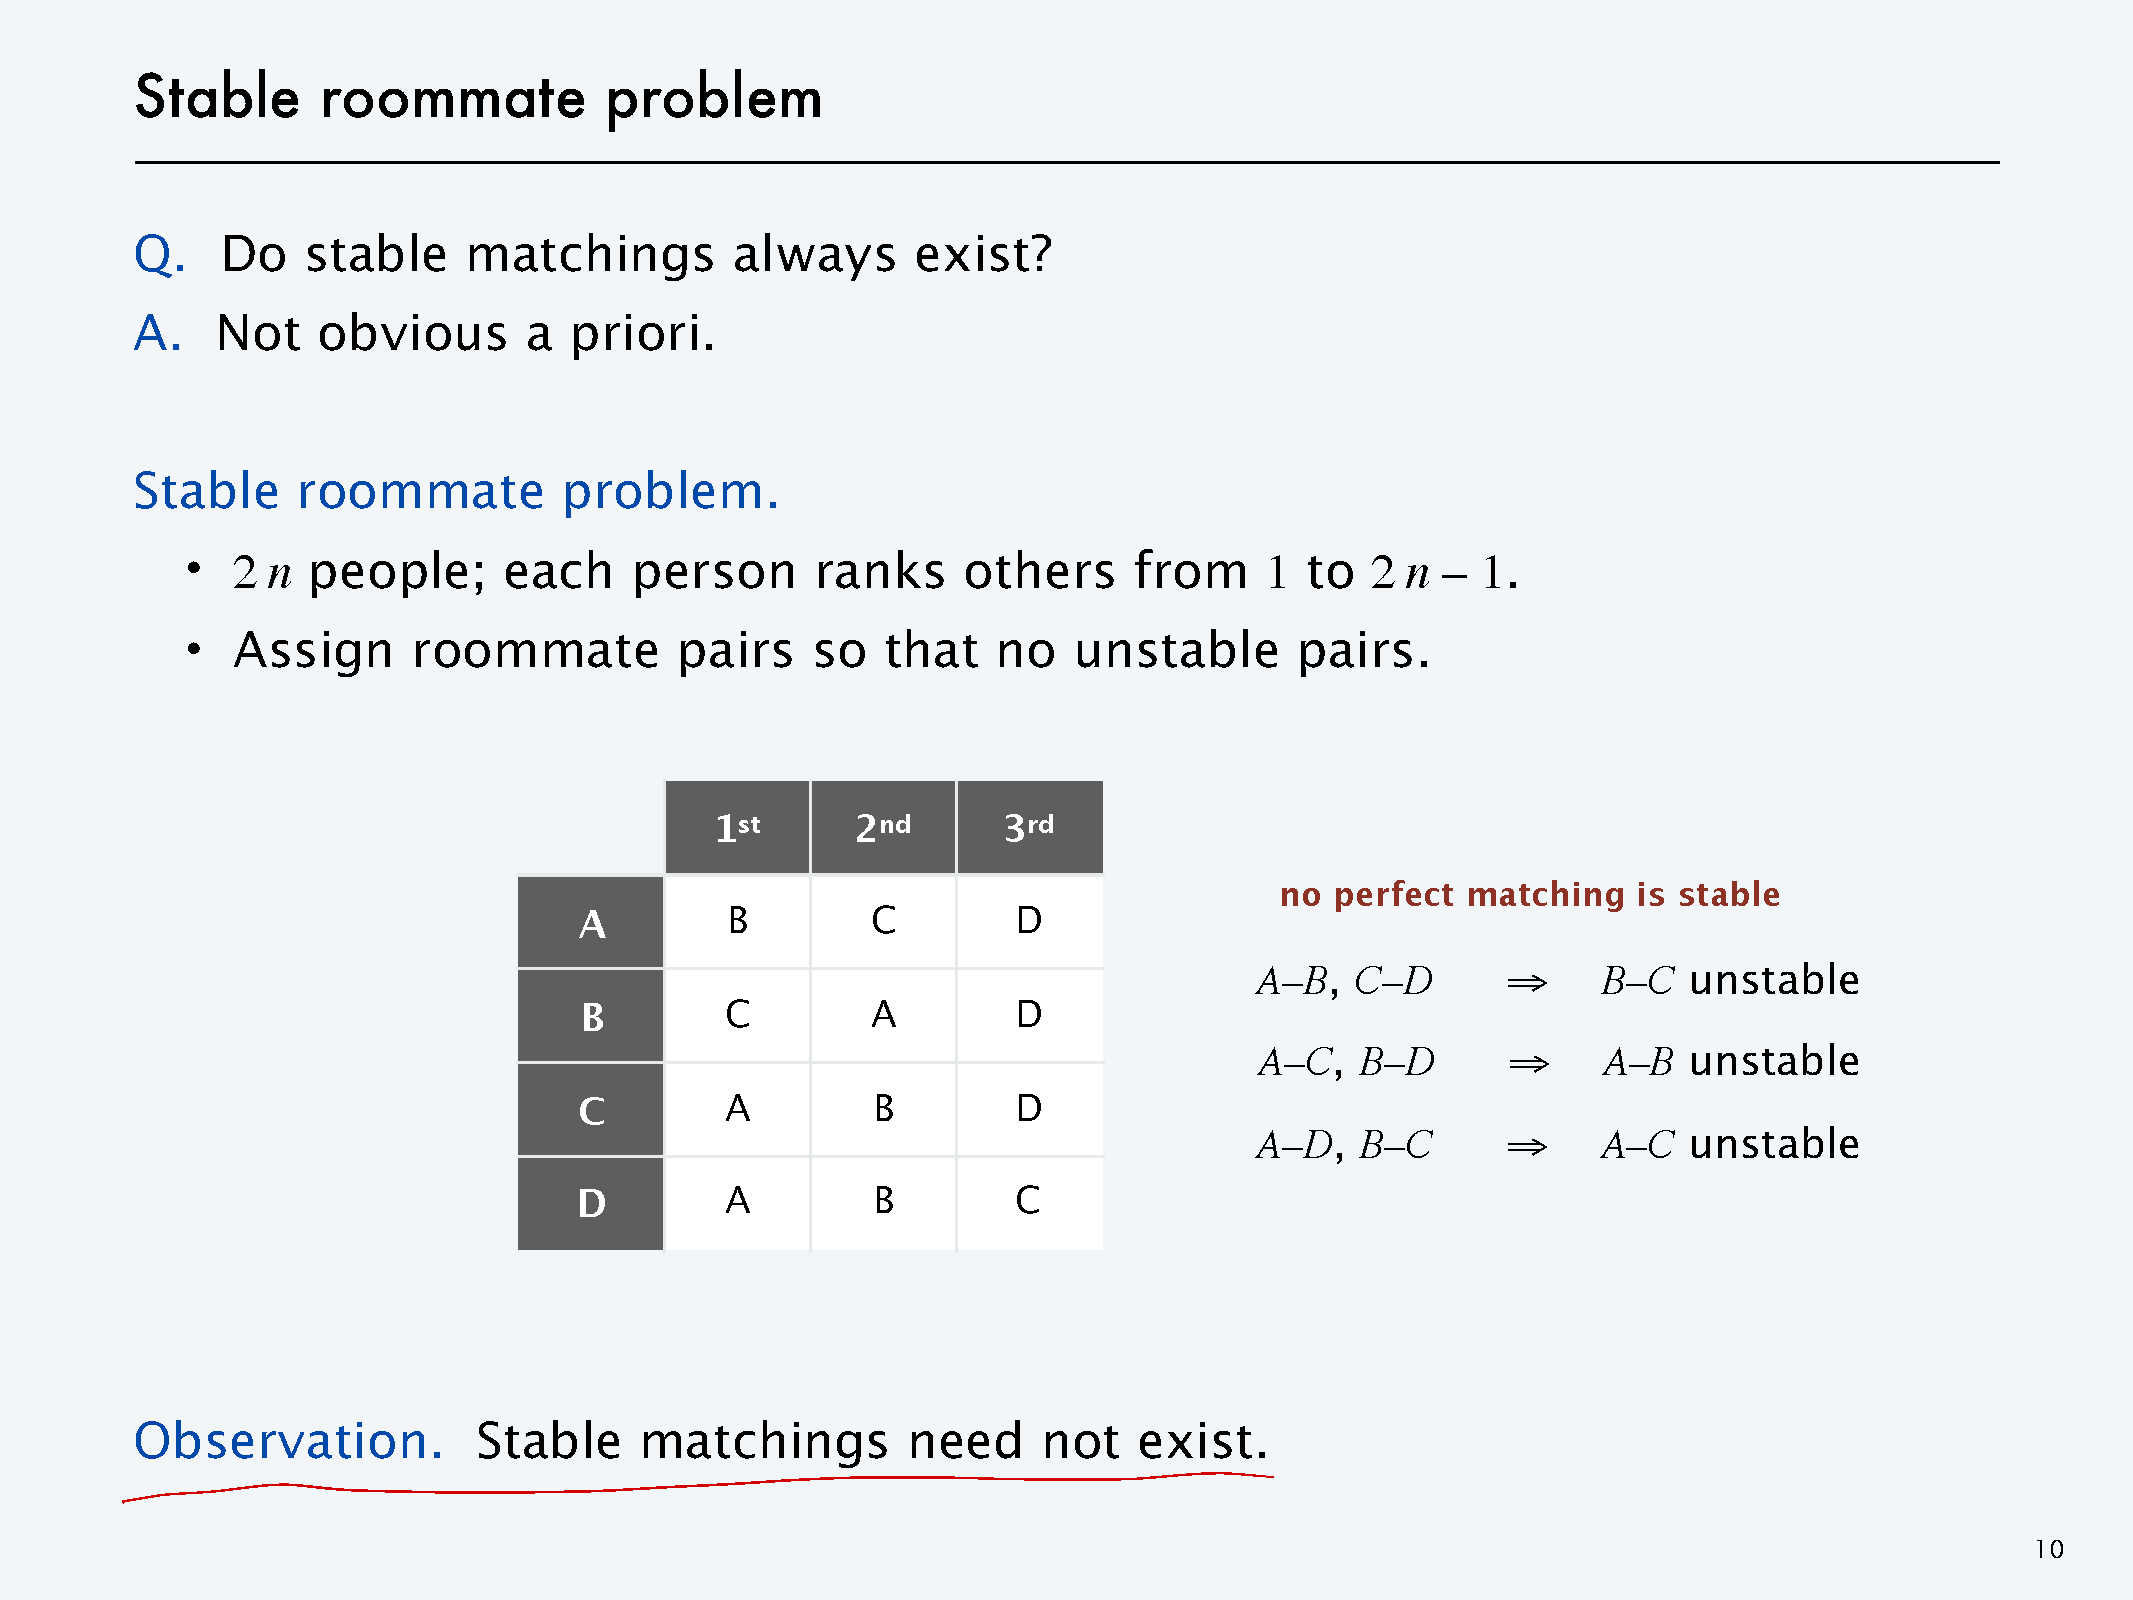
\includegraphics[scale=0.37]{1.pdf}
\end{figure}

\subsection{Kleinberg and Tardos, Chapter 1, Exercise 4}

\begin{algorithm}
        \caption{Extended Gale-Shapley Algorithm}
        \begin{algorithmic}[1] %每行显示行号
                \State Initially all $r\in R$ and $h\in H$ are free
                \While{some hospital $h$ has a vacant position \textbf{and} $h$ hasn't asked every student}
                \State Choose such a hospital $h$
                 \State Let $s$ be the highest-ranked student in $h$'s preference list to whom $h$ has not yet asked
                    \If{$s$ is free then}
                        \State assign $s$ provisionally to $h$
			\Else {$s$ is currently assigned to $h'$}
                     	\If{$s$ prefers $h$ to $h'$}
			\State assign $s$ provisionally to $h$
			\State remove $s$ from $h'$ positions.
			\EndIf
                    \EndIf
         \EndWhile
        \end{algorithmic}
\end{algorithm}

On termination each undersubscribed hospital has assigned to it all of the students on
its reduced list, and a fully assigned hospital with $q$ places has assigned to it the first $q$ students on its reduced list.

It can be shown that the matching defined by the provisional assignments on
termination is uniquely defined for any given instance of the problem and that it is
stable. If a hospital is undersubscribed, no other student is assigned to it in any stable
matching. Also, each student is assigned in this matching to his worst valid partner.

\subsection{N men and N women were participating in a stable matching process in a small town named Walnut Grove.}

Let's simplify this problem as a man-propose process.

First of all, Almazo will propose to Laura, if Laura decides to reject him and stay with her current fiance(let's say Ben), then Almazo will just simply turn back to Nelly.

However, if Almazo ranks higher than Ben in Laura's preference list, then Laura will accept Almazo as fiance, leaving Nelly and Ben back to single situation.

Since Nelly remains alone for now, those men who ranks Nelly higher than their current partner will step out and propose to Nelly, there comes two situations: 1. If there's no one who prefers Nelly than their partner, then Nelly will still remains alone; 2. If it does exist such a group of men, then Nelly will choose the best one according to her preference. Let's say Nelly chooses Allen, and Allen breaks up with his girlfriend, Alice.

Eventually, the single woman will face the first situation: that is no man who prefers her than his current partner. Let's just suppose Alice is the girl who confronts such awkward situation, what she can do now is to wait and some man to take her hand.

In the meantime, Ben will decide who he will propose to, is it the one who remains alone right now or propose to someone who has paired up. If the single woman ranks higher than Laura, then Ben can just pair up with her. However if she ranks lower than Laura, then he'll have to search all the way down his preference list. Notice that Ben can only pair with those ranks lower than Laura and higher than single woman according to his preference. Suppose Ben successfully paired up with Cindy, and made Bob a bachelor.

Now that the same situation will happens on Bob: to propose to single woman or the others. If he successfully proposed to another woman, then the bachelor identity will switch to another man; However if Alice happens to rank higher than Cindy(Bob's previous partner), then Bob will propose to Alice, the algorithm comes to an end.

To conclude, each iteration of the algorithm takes 5 steps:
\begin{itemize}
\item 1. Each iteration begins with a single woman $W$ and a single man $M$
\item 2. List out all the man who prefers $W$ than his current partner, if $M$ is inside this list, jump out step 3. $W$ will choose the best one according to her preference. If the list is empty, continue.
\item 3. According to $M$'s preference list, propose to the next woman.
\item 4. If $W$ pairs up with $M$, algorithm stops and quits.
\item 5. Renew $W$ and $M$.
\end{itemize}


\section{Practice Problems}

\subsection{Kleinberg and Tardos, Chapter 1, Exercise 1.}

False. Consider a following situation: the arrow indicates the preference (over another person):

\begin{figure}[H]
\centering
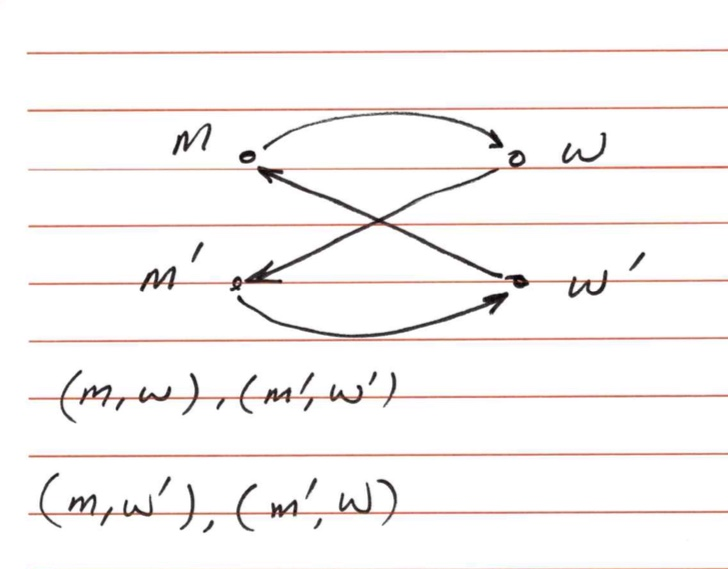
\includegraphics[scale=0.37]{1.jpeg}
\end{figure}

Two possible perfect matching does not include the such pair satisfying the condition stated in the topic.

\subsection{Kleinberg and Tardos, Chapter 1, Exercise 2.}

True. Imagine if a stable matching $S'$ does not include pair $(m, w)$. Suppose $(m, w')\in S$, $(m', w)\in S$. Then $(m, w)$ is an unstable pair, $S$ is not a stable matching. Therefore, for all possible stable matching, $(m, w)$ is sure to be one of its element.

\subsection{Kleinberg and Tardos, Chapter 1, Exercise 3.}

There is not always a stable pair of schedules given a set of TV shows and ratings.

For instance, Suppose A has two shows ($a_1, a_2$) with ratings of 2 and 4, and B has two shows $(b_1, b_2)$ with ratings of 1 and 3. Then there are two possible schdules: $(a_1, b_1), (a_2, b_2)$ or  $(a_1, b_2), (a_2, b_1)$. In the first situation, B will consider switch the two shows in order to win one slot; While in the second situation, A will switch two shows to win both slots rather than only one. Therefore, no matter what the situation is, there will always exist one network who wishes to change its schedule, this is an counterexample. 






\end{document}